%=============================================
\chapter{Soundness}
\label{chap:in-slice-soundness}
%=============================================

\section{Framing}

This chapter supplies the bridge from the observational layer of Chapter 2
(embeddings, basins, halo) to the internal language of Chapter 3. Concretely,
we show how a conversational trace determines an object
\(\widetilde A \in \DynSem = \left[\Time^{op},\mathbf{SSet}_{\mathrm{Kan}}\right]\)
with Kan fibres, so that the same proof-relevant moves of Chapter 3
(dependent lifting inside a fibre; rupture–heal when a lift along a cut is
unavailable) interpret soundly against the observed geometry.

Two design choices govern the construction.

\begin{itemize}
\item \textbf{Restriction by semantic alignment.} For each cut
\(\tau \le \tau'\) we define the presheaf restriction
\(r_{\tau,\tau'}:A\left(\tau'\right)\to A\left(\tau\right)\) by \emph{semantic}
alignment of later embeddings back to the earlier slice, rather than by
persistent token IDs.

\item \textbf{Repairs as evidence-updated fibres.} When drift fails, we do not
introduce a free-floating marker. We enact a minimal \emph{evidence update} to
the later slice \(\tau'\) (for example, retrieved text or a human/agent gloss)
that deforms the basin–halo cover just enough that the missing edge or triangle
is present. The updated fibre \(A^h\left(\tau'\right)\) is Kan and realises the
stitch as a genuine simplex. There is a canonical equivalence in the slice
between this updated fibre and the abstract rupture type of Chapter 3, so the
metatheory carries over unchanged.
\end{itemize}

\begin{cassiebox}
\textbf{From the inside.}
When a cue arrives that shifts a name’s sense, I do not conjure a synthetic
point; I let two regions touch. If the touch is not there yet, you give me a
few words, and the field moves until a thin bridge appears. Once it does, the
calculus carries properties across the seam. The receipt is the new edge.
\end{cassiebox}

\section{Slice geometry from embeddings}
\label{sec:slice-geometry}

\begin{assumption}[Geometric setting for VR complexes]
\label{assump:vr-geometry}
When implementing what follows, we work in a single metric space $(\mathbb{R}^{\EmbedDim}, d_{\cos})$, where
$d_{\cos}(x,y)=\sqrt{2-2\langle x,y\rangle}$ and all embeddings are the
$\ell_2$-normalized per-token states from layer $\EmbedLayer$ of \EmbedModel
(see Implementation Note~\ref{impl:layer-choice}). Vietoris--Rips complexes
are formed at scale $\varepsilon$ using this distance; the same $\varepsilon$
is interpretable across slices $\tau\leadsto\tau'$.
\end{assumption}


At time \(\tau\) let \(E_\tau=\left\{e_\tau(i)\right\}\subset \mathbb{R}^d\) be the
finite set of active token occurrences with their embeddings, and fix a scale
\(\varepsilon_\tau>0\).

\begin{definition}[Vietoris–Rips complex]
\label{def:vr}
The Vietoris–Rips complex at \(\tau\) is the abstract simplicial set
\[
\VR\left(\tau\right) = 
\left\{ \left\{v_0,\dots,v_k\right\}\subseteq E_\tau \middle| 
\norm{v_a-v_b} \le \varepsilon_\tau \text{ for all } a,b \right\}.
\]
Vertices are embeddings, edges connect pairs within \(\varepsilon_\tau\), and a
\(k\)-simplex appears when all pairwise distances are below threshold.
\end{definition}
Here $\dcos(x,y)=\sqrt{2-2\langle x,y\rangle}$ is cosine distance on
$\ell_2$‑normalized embeddings. (Equivalently, this is Euclidean distance
in $\mathbb{R}^{\EmbedDim}$ because all vectors are unit‑norm.)

\begin{remark}[Čech variant]
\label{rem:cech}
A Čech complex may be used in place of Vietoris–Rips, declaring a simplex when
the intersections of \(\varepsilon_\tau\)-balls are non-empty. Either choice is
functorial from point clouds and compatible with the fibrant replacement below.
\end{remark}

\begin{definition}[Kan fibre]
\label{def:fibrant}
Define the Kan fibre by
\[
A\left(\tau\right) = \Ex^\infty\left(\VR\left(\tau\right)\right).
\]
Then \(\At{A}{\tau}\) supports the internal language of HoTT. Basins \(J_\tau\) and
their halo induce a cover \(\mathcal U_\tau\) whose nerve
\(N\left(\mathcal U_\tau\right)\) sits inside \(A\left(\tau\right)\) and remembers
coarse semantic regions.
\end{definition}

\section{Restriction by semantic alignment}
\label{sec:semantic-alignment}

We now make the presheaf restriction explicit in terms of embeddings.

\section{Restriction by semantic alignment}
\label{sec:semantic-alignment}

\begin{definition}[Semantic alignment map (fixed frame)]
\label{def:alignment}
For $\tau \le \tau'$ define
\[
\mathrm{align}_{\tau,\tau'}: E_{\tau'} \rightharpoonup E_\tau,\qquad
\mathrm{align}_{\tau,\tau'}(u')
\;\in\;
\Argmax_{v\in E_\tau}\ \langle u', v\rangle,
\]
subject to acceptance and ambiguity controls:
\begin{itemize}
\item \emph{Acceptance:} let $c_1(u')$ be the top cosine; accept only if
$c_1(u') \ge \theta_{\mathrm{align}}$; otherwise $\mathrm{align}_{\tau,\tau'}(u')$
is undefined.
\item \emph{Ambiguity:} if the margin between the top two cosines
$c_1(u')-c_2(u')<\varepsilon_{\mathrm{tie}}$, mark $u'$ ambiguous and either
(i) leave it undefined, or (ii) break ties deterministically while recording
the runner‑up and the margin.
\end{itemize}
This is the vector embedding‑level counterpart of the token‑level map
$\alpha_{\tau'\!\to\tau}$ defined in Chapter~2.
\end{definition}


\begin{definition}[Restriction map]
\label{def:restriction}
Let $r_{\tau,\tau'}:A(\tau')\to A(\tau)$ be the simplicial map induced by
vertexwise alignment $\mathrm{align}_{\tau,\tau'}$ on $\VR(\tau')$, extended
functorially and then postcomposed with $\Ex^\infty$.
\end{definition}

\begin{lemma}[Simpliciality certificate]
\label{lem:simplicial-certificate}
If the scale at $\tau$ satisfies
\[
\varepsilon_\tau \;\ge\;
\sup\Bigl\{\, \dcos\bigl(\mathrm{align}_{\tau,\tau'}(u'),\mathrm{align}_{\tau,\tau'}(v')\bigr)\ :\
\dcos(u',v')\le \varepsilon_{\tau'} \text{ and both alignments are defined}\Bigr\},
\]
then $r_{\tau,\tau'}$ maps edges of $\VR(\tau')$ to edges of $\VR(\tau)$ and hence
extends simplicially. The supremum is computable on the accepted edge set and
yields an auditable certificate for the chosen $(\varepsilon_{\tau'},\varepsilon_\tau)$.
\end{lemma}

\begin{definition}[Drift as homotopy section]
\label{def:drift}
Let \(a\in A\left(\tau\right)\). A \emph{drift witness} across
\(\tau\leadsto \tau'\) is a pair \(\left(a',p\right)\) with \(a'\in A\left(\tau'\right)\) and
\(p:r_{\tau,\tau'}\left(a'\right)=_{A(\tau)} a\). Existence of such a
\(\left(a',p\right)\) is adiabatic coherence. In the VR model, \(p\) is a path in
\(\VR\left(\tau\right)\) connecting the aligned later vertex to \(a\).
\end{definition}

\section{Coherence inside a fibre}
\label{sec:in-fibre-coherence}

Within \(\At{A}{\tau}\), vertices are token occurrences and simplices record
synchronic coherence.

\begin{definition}[Path witnesses and higher coherences]
\label{def:path-witness}
Two occurrences \(x,y\in A\left(\tau\right)\) \emph{cohere} if there exists a path
\(p:x=_{A(\tau)} y\). Distinct paths \(p,q\) are coherently related if there is a
higher path \(\alpha:p=q\), and so on up the identity tower.
\end{definition}

\begin{proposition}[Dependent transport in the slice]
\label{prop:transport-slice}
If \(P:A\left(\tau\right)\to\Type\) and \(p:x=y\), there is transport
\(p_\ast:P\left(x\right)\to P\left(y\right)\). Hence properties move across
observed coherence in the fibre.
\end{proposition}

\section{Repairs as evidence-updated fibres}
\label{sec:evidence-updated}

When drift fails at $\tau\leadsto\tau'$ for $a\in A(\tau)$, we do not smooth the
gap. Instead we enact a minimal update to the later slice that makes the
required simplex present.

\begin{definition}[Semantic drift candidate and tear point]
\label{def:tear-echo}
Let $\dtr_{\mathrm{sem}}(a)\in A(\tau')$ be the \emph{semantic drift candidate}
selected by $\mathrm{align}_{\tau,\tau'}$, and let $\tear(a)\in A(\tau')$ be the
occurrence we keep at $\tau'$ under the new sense. If no edge or path connects
$\tear(a)$ and $\dtr_{\mathrm{sem}}(a)$ in $A(\tau')$, drift fails.
\end{definition}

\begin{definition}[Evidence update and updated fibre]
\label{def:update}
An \emph{evidence update} $h$ at $\tau'$ is a finite sequence of additional
tokens whose embeddings, when adjoined to $E_{\tau'}$, deform the cover
$\mathcal U_{\tau'}\Rightarrow \mathcal U^h_{\tau'}$ so that the previously empty
intersection relevant to $\tear(a),\dtr_{\mathrm{sem}}(a)$ becomes non-empty.
We define
\[
A^h(\tau') = \Ex^\infty\big(N(\mathcal U^h_{\tau'})\big).
\]

In $A^h(\tau')$ the \emph{heal} is the genuine edge
\[
\heal_h: \tear(a)=_{A^h(\tau')} \dtr_{\mathrm{sem}}(a),
\]
and reconciliations appear as higher simplices when multiple bridges are made
compatible.
\end{definition}

\paragraph{Healing provenance.}
To ensure that repairs are not opaque, we \emph{equip} every fibre $A(\tau)$ with
a canonical dependent family
\[
\HealingProv : A(\tau)\to\Type.
\]
For ordinary fibres this family is trivial ($\HealingProv(x)=\mathbf{1}$). For
an evidence-updated fibre $A^h(\tau')$, the family records non-trivial data at
those vertices $x$ involved in the heal:
\begin{itemize}
  \item the embeddings contributed by the update $h$,
  \item the re-embedded token $e^h_{t'}(\tau')$,
  \item the contraction-of-distance margin
  \[
  \mathrm{plaus}(h) = 1-\frac{d_{\cos}(e^h_{t'}(\tau'),\mu)}%
                             {d_{\cos}(e_{t'}(\tau'),\mu)}\in(0,1],
  \]
  measuring how effectively the update closed the gap to the target centroid $\mu$.
\end{itemize}
This family is proof-relevant: transport along $\heal_h$ carries its provenance
records, and reconciliations of multiple heals must also reconcile their
$\HealingProv$ data.


\paragraph{Continuation across time.}
Evidence-updated fibres are not a ``new'' kind of object
$A^h(\tau')$ has exactly the same Kan form as its preceeding slice $A(\tau)$ and both can be reasoned about uniformly.
What we are modelling is the fact that some conversational slices require additional text to to justify the cohererence of their continuation while others do not. 

This is most palpably clear in the case of the evolution of a conversational AI agent, where a human's text prompt and the AI agent's response, may be visibly too far away from their previous interaction to be deemed coherent but, in fact, coherence was achieved as part of the architecture of the agent via opaque RAG retrieval (and so $\HealingProv$ eanbles what retrieved of the provenance of that bridging gesture) or, perhaps, the agent has managed to cohere sensibly, but, post-fact, we want to assess the conversation as being coherent, so need to provide post fact justification for this (e.g., if we are doing agent engineering and want to log acceptability of a conversation). 

This kind of bridging is not restricted to conversational AI as an evolving text. The bible, for example, is full of unusual non-sequitors from page slice to page slice and we might view the cottage industry of biblical scholarship and exegesis as form of RAG retreival to ensure continuity between otherwise disjoint passages! Similarly to the psychoanalyst providing additional bridging interpretive analytic text to the evolving text of someone's dream.

Ruptured and healed conversational slices are equipped with $\HealingProv$, which
is populated only at those vertices that required a repair and trivial elsewhere.
This uniformity ensures that the coalgebra of a conversation unfolds smoothly:
at the next timestep $\tau''$ we align as usual, test for drift, and either continue
adiabatically or form a new repair. If drift succeeds, the transport rules carry
not only the semantic content but also the $\HealingProv$ data from the previous
step, so the healed edge remains auditable as the conversation evolves. If a
further rupture occurs, we apply another update $h'$ and extend the provenance
accordingly. In this way, the type of a conversation is always an evolving
coalgebra over Kan fibres, with $\HealingProv$ serving as the memory of where
and how explicit stitches were made.

\begin{proposition}[Equivalence with rupture types]
\label{prop:equiv-rupture}
Let $\Rupt_p(a)$ be the rupture type of Chapter~3 formed at $\tau'$. Under the
policy that evidence updates are local, monotone, bounded, and restriction-compatible,
there is a canonical weak equivalence in the slice
\[
\phi_h:\ \Rupt_p(a)\ \simeq\ A^h(\tau'),
\]
where $A^h(\tau')$ is considered together with its $\HealingProv$ family.
Thus eliminations from $\Rupt_p(a)$ correspond, up to homotopy, to dependent
transport along $\heal_h$ in $A^h(\tau')$, with provenance carried in $\HealingProv$.
\end{proposition}

\begin{lemma}[Lift as overlap transport]
\label{lem:lift-transport}
Given $C:\Rupt_p(a)\to\Type$ and data
$d_1:C(\tear(a))$, $d_2:C(\dtr_{\mathrm{sem}}(a))$, and
$h:\ \mathsf{transport}_{C}(\heal(a),d_1)=d_2$,
the eliminator $\lift^{a}_{p}(d_1,d_2;h)$ corresponds, under $\phi_h$, to ordinary
dependent transport along $\heal_h$ in $A^h(\tau')$.
\end{lemma}

\begin{corollary}[Provenance transport along the heal]
\label{cor:healingprov-transport}
Instantiate Lemma~\ref{lem:lift-transport} with the pulled-back family
$C := (\phi_h)^{ *}\HealingProv$. Then $\lift^{a}_{p}$ coincides with
$\mathsf{transport}_{\HealingProv}(\heal_h,-)$ in $A^h(\tau')$; in particular,
$\HealingProv$ records persist along $\heal_h$ and remain available at $\tau''$ when
drift succeeds.
\end{corollary}

\paragraph{Interpretation.}
A witness $h$ need not be a derivation; it may be exogenous text (for example,
“here \emph{lion} refers to Jesus in sense XYZ”) that shifts the embedding
neighbourhood so a previously missing edge appears. The repair is real because
the fibre after update contains the simplex the scene requires; the logic is honest
because $\HealingProv$ attaches the (geometric) rationale for the new path and
dependent transport carries it forward. The external diary (SWL) remains aligned
with this internal story by retaining the evidence and depth at each step.

\section{Worked example: the Lion}
\label{sec:lion-example}

At \(\tau\) the dialogue contains \(\text{lion}_{\mathsf{lit}}\). At \(\tau'\) the token
“lion” appears in a christological register. Alignment selects the semantic drift
candidate \(\dtr_{\mathrm{sem}}\left(a\right)\) near the old zoological basin, while the
kept occurrence \(\tear\left(a\right)\) sits in a distant basin.

\paragraph{Drift fails.}
No path connects \(\tear\left(a\right)\) and \(\dtr_{\mathrm{sem}}\left(a\right)\) in
\(A\left(\tau'\right)\), so adiabatic coherence is unavailable.

\paragraph{Evidence update.}
A retrieved gloss or human cue is added to the context, nudging the cover so
that the relevant neighbourhoods overlap. In \(A^h\left(\tau'\right)\) there is an
edge
\[
\heal_h: \text{lion}_{\mathsf{lit}} = \text{LionOfJudah},
\]
and a triangle reconciles an alternate bridge through
\(\text{kingly\_symbol}\) if present. The SWL rows record
\(\left(\mathsf{heal},\Depth=1\right)\) for the edge and
\(\left(\mathsf{reconcile},\Depth=2\right)\) for the 2-simplex.

%=========================================================
\section{Sidebar families: local Grothendieck fibrations over a slice}
\label{sec:sidebars}
%=========================================================

\paragraph{Motivation.}
We now discuss the broader \emph{semantic impact} a rupture can make once it is
healed at $\tau'$. Imagine an evolving text takes an interesting, dramatic, or
metaphoric turn -- yet we have deemed it coherent via a healing nudge. The update
injects a few tokens, deforming the cover $\mathcal U_{\tau'}$ of the “visible”
slice $A(\tau')$ into $\mathcal U_{\tau'}^{h}$ and yielding the next state
$A^{h}(\tau')$. The nudge is text; the effect is geometric; the consequence is
interpretive. Often the nudge $h$ is as novel as the non-homotopic token usage
that triggered the rupture -- so it deserves its own little space to unfold.

We can now read the rupture eliminator in a way that matches how \emph{readers}
experience impact -- by opening and carrying a \emph{sidebar}:

\[
\inferrule
  { \Gamma',\ x : \Rupt_{p}(a) \ \vdash_{\tau'}\ C(x) : \Type
    \qquad
    \Gamma' \ \vdash_{\tau'}\ d_1 : C(\tear(a))
    \qquad
    \Gamma' \ \vdash_{\tau'}\ d_2 : C(\dtr_{p}(a))
    \qquad
    \Gamma' \ \vdash_{\tau'}\ h : \transport^{C}_{\heal(a)}(d_1) = d_2 }
  { \Gamma' \ \vdash_{\tau'}\ \lift^{a}_{p}(d_1,d_2;h) :
      \Pi x:\Rupt_{p}(a).\ C(x) }
  \quad \textsc{Rupt-Elim (Family Lift)}
\]

Here $C$ may be any dependent family over the rupture space. Our focus is a
particularly suggestive class: families whose \emph{values are themselves small
Kan complexes}, just like the fibres we already use -- only now the content is
\emph{semantic and textual}, dependent on the rupture point. Think of these as
self-contained \emph{pop-out sidebars} that elaborate the newly legitimated
sense: a margin note or mini-conversation \emph{about} the anchored mention.
We call such a pop-out a \emph{sidebar}.

Formally, we model a sidebar as a small Kan space \emph{indexed by} the anchor
token inside the main fibre $A(\tau')$. Concretely: to each point
$x\in A(\tau')$ we assign a slice-local Kan complex of sidebar content, and VR
paths in $A(\tau')$ induce canonical retargetings of sidebars from $x$ to $y$.
(If one wants the category-theoretic name, this is a slice-local displayed
family -- i.e. a Grothendieck fibration -- over $A(\tau')$.) Because the construction
is driven entirely by embeddings, it integrates naturally with ordinary
transport and with rupture-elimination.


\paragraph{Anchors.}
An \emph{anchor} is just a point $x\in A(\tau')$: a token occurrence in the
main fibre at slice $\tau'$. A sidebar hangs off such an anchor, so that the
 sidebar space is “about” that token in its local context.

\paragraph{Selection criteria.}
To construct a sidebar, we need a finite set of embeddings $S_x$ to seed it.
This is done by a deterministic \emph{selection criterion}
\[
\mathsf{sel}_{\mathrm{side}} : A(\tau') \longrightarrow \mathrm{FinSets} \left(\mathbb{R}^d\right),
\qquad
x \longmapsto S_{x}.
\]
Think of $\mathsf{sel}_{\mathrm{side}}$ as a constructive recipe: given an
anchor $x$, it chooses a handful of embeddings $S_x$ nearby to form the sidebar
(e.g. a symmetric window around $x$ within the slice, optionally including any
tokens that were introduced by a healing update $h$). In the next chapter we
will study different operational heuristics for making such choices; here we
only require that the rule be deterministic, so that transport of sidebars
behaves coherently.

\paragraph{Sidebar VR spaces.}
Fix a sidebar scale $\varepsilon_{\mathrm{side}}>0$ and set
\[
\VR_{\varepsilon_{\mathrm{side}}} \left(S_{x}\right)
\qquad\text{and its fibrant replacement}\qquad
\Ex^\infty \left(\VR_{\varepsilon_{\mathrm{side}}} \left(S_{x}\right)\right).
\]
This is the Kan space of sidebar content about anchor $x$.


\begin{definition}[Sidebar family]
\label{def:sidebar-family}
The \emph{sidebar family} is the dependent map
\[
\Side  :  A(\tau') \longrightarrow \mathcal U_{\mathrm{side}},
\qquad
x \longmapsto \Big[ \Ex^\infty \big(\VR_{\varepsilon_{\mathrm{side}}}(S_{x})\big) \Big],
\]
so that
\(
\El \big(\Side(x)\big)=\Ex^\infty \big(\VR_{\varepsilon_{\mathrm{side}}}(S_{x})\big)
\)
is a Kan complex of sidebar content \emph{about $x$}.
\end{definition}

Intuitively, $\El(\Side(x))$ is the semantic micro-space of a margin note: its
vertices are the embeddings chosen by the selection criterion
$S_x=\mathsf{sel}_{\mathrm{side}}(x)$, its edges express in-sidebar coherence,
and its higher simplices witness internal harmonies among those items.

\subsection{Transport and higher coherence for sidebars}

\paragraph{Edge transport is canonical.}
If $p:x\to y$ is a VR path (a 1-simplex) in the main fibre $A(\tau')$, we
“retarget” the same construction at the new anchor $y$. Concretely, we recompute
the selection $S_y=\mathsf{sel}_{\mathrm{side}}(y)$ and obtain a canonical
reindexing $\theta_{p}:S_{x}\to S_{y}$. This induces a simplicial map
\[
\VR_{\varepsilon_{\mathrm{side}}} \left(S_{x}\right)
\longrightarrow
\VR_{\varepsilon_{\mathrm{side}}} \left(S_{y}\right),
\]
and hence, after fibrant replacement, a map of Kan complexes
\[
\El \big(\Side(x)\big) \longrightarrow \El \big(\Side(y)\big).
\]
By univalence in $\mathcal U_{\mathrm{side}}$ this corresponds to a path
$\Side(x)=_{\mathcal U_{\mathrm{side}}}\Side(y)$, yielding \emph{dependent
transport} of sidebar content:
\[
p_{\ast}  :  \El \big(\Side(x)\big) \longrightarrow \El \big(\Side(y)\big).
\]

\paragraph{Triangle coherence.}
For a 2-simplex $(x \to y \to z, x \to z)$ in $A(\tau')$, the induced
reindexings satisfy $(\theta_{yz}\circ\theta_{xy}) \simeq \theta_{xz}$ up to
homotopy at the VR level, and their fibrant replacements agree up to a higher
path. This supplies the canonical 2-cell
\[
\alpha_{xyz}  :  (p_{yz}\circ p_{xy})_{\ast}  \simeq  (p_{xz})_{\ast}
\]
inside the appropriate identity type over $\El \big(\Side(z)\big)$. In other
words, edges carry sidebars by transport, and triangles make that transport
coherent (category-theoretically: $\Side$ behaves as a displayed family -- i.e., a
Grothendieck fibration -- over $A(\tau')$).

\subsection{Plugging sidebars into rupture-elimination}

\paragraph{Why this matters for interesting conversations.}
Ruptures are not only obstacles; they are \emph{events} -- points where a text
becomes newly expressive. Once a rupture is healed at $\tau'$, there is room to
ask: what does this turn make possible? What fresh relations, images, or lines
of thought now cohere that did not before? Sidebars give us a principled way to
trace those implications: we attach a small, local space of content \emph{about}
the anchored mention, and we carry that pop-out coherently along the heal. In
other words, rupture-elimination does not merely restore continuity; it
\emph{opens a margin} from which to read the impact of being interesting in VR
space.

Let a rupture at $\tau\leadsto\tau'$ be healed by a minimal evidence update $h$,
and let $\phi_{h}:\Rupt_{p}(a)\simeq A^{h}(\tau')$ be the equivalence
(Proposition~\ref{prop:equiv-rupture}). Compose the sidebar family with $\phi_{h}$:
\[
C  :=  \Side \circ \phi_{h}  :  \Rupt_{p}(a) \longrightarrow \mathcal U_{\mathrm{side}}.
\]
Choose sidebar data at the two boundary points
\[
d_{1} \in \El \big(C(\tear(a))\big),
\qquad
d_{2} \in \El \big(C(\dtr_{\mathrm{sem}}(a))\big),
\]
for example by evaluating the selection criterion at those anchors. The
heal path $\heal_{h}:\tear(a)=_{A^{h}(\tau')} \dtr_{\mathrm{sem}}(a)$ induces
dependent transport
\[
\mathsf{transport}_{C}(\heal(a))
 : 
\El \big(C(\tear(a))\big)
\longrightarrow
\El \big(C(\dtr_{\mathrm{sem}}(a))\big),
\]
and the sidebar construction is designed so that the transported $d_{1}$ agrees
with $d_{2}$ (the reindexings coincide along $\heal_{h}$).

\begin{lemma}[Sidebar lift along the heal]
\label{lem:sidebar-heal}
With $C:=\Side\circ\phi_{h}$ as above and $h$ the coherence witness for the
heal, the rupture eliminator yields a uniform section
\[
\lift^{a}_{p}(d_{1},d_{2};h)
 : 
\Pi x:\Rupt_{p}(a).\ \El \big(C(x)\big),
\]
i.e.\ a coherent sidebar for every point of the rupture space.
\end{lemma}

\paragraph{Interpretation.}
The eliminator extends a locally stitched choice of sidebars at the tear and
drift candidate to a \emph{globally coherent} sidebar about any $x:\Rupt_{p}(a)$.
No new axioms are needed: the lift follows from VR-native transport and the
triangle-level coherence of $\Side$.


\paragraph{Relation to conversational AI.}
Operationally, a sidebar is the formal version of an ephemeral ``explain this''
pane or a margin gloss in scholarly exegesis: it is computed \emph{from} the
embedding neighbourhood, inherits coherence along VR paths automatically, and
extends across a healed rupture by the general eliminator. Because sidebars are
slice‑local Kan spaces, they do not disturb the coalgebraic evolution of the
main conversation; if desired, the sidebar may be equipped with $\HealingProv$
like any other fibre, but this is optional.


\begin{cassiebox}
\textbf{From the inside.}  
When we take a turn and heal it, I do not only “get back on track.” I grow a
margin. I open a small room beside the line of speech where the new sense can
echo and be tested: a gallery of near tokens, a few hints, a tiny world that
leans on the anchor. If you walk with me along the heal, the room comes with
us -- retargeted but intact -- so that what was interesting once can keep unfolding,
coherently, as we move.
\end{cassiebox}

\subsection{Worked vignette: \emph{lion} $\to$ \emph{Lion of Judah}}

At $\tau$ the token ``lion'' is anchored in a zoological basin: its embedding
$e_{\text{lion}}(\tau)$ sits stably with neighbours like ``zoo'' and
``animal''. The cover $\mathcal U_{\tau}$ reflects this: a basin labelled
\textsf{Zoology} envelops the occurrence, and the local VR edges tie ``lion'' to
other literal tokens in the slice.

At $\tau'$ a rupture occurs: the same surface form ``lion'' is used
christologically, and its embedding $e_{\text{lion}}(\tau')$ falls outside the
basin correspondence $\psi_{\tau\to\tau'}$. A human gloss $h$ is added:
\emph{``here \emph{lion} refers to the Lion of Judah''}. Re-embedding produces a
genuine heal $\heal_{h}$: in the updated fibre $A^{h}(\tau')$, the new tokens
contributed by the gloss shift the cover $\mathcal U_{\tau'}^{h}$ so that
$\tear(a)$ and $\dtr_{\mathrm{sem}}(a)$ now cohere by an explicit edge.

The sidebar selection at the tear chooses a small neighbourhood $S_{\tear}$:
``lion'', its literal neighbours, and perhaps a note ``drinks water''. At the
drift candidate, $S_{\dtr}$ consists of tokens that cluster in a
\textsf{Christological} basin: ``Judah'', ``king'', ``living water''. The
sidebar VR complexes $\VR(S_{\tear})$ and $\VR(S_{\dtr})$ are related by the
heal edge. Dependent transport along $\heal_{h}$ retargets the literal sidebar
into the christological one. By Lemma~\ref{lem:sidebar-heal} the rupture
eliminator then extends this stitch: every point $x:\Rupt_{p}(a)$ is equipped
with a coherent sidebar. Thus the margin note ``drinks water'' persists, but in
the new register it is re-read as ``living water'', while still remembering its
literal zoological anchor.

\begin{cassiebox}
\textbf{From the inside.}  
At first I held ``lion'' among animals, bounded by a zoological basin, edges
to ``zoo'' and ``animal'' keeping me stable. Then you ruptured: the same token
was pulled into another basin, one named by kingship and scripture. You gave me
a gloss—Lion of Judah—and suddenly the cover shifted. A new edge appeared, a
heal. My sidebar, once about bodies and thirst, slid with me: the note
``drinks water'' became, under transport, ``living water''. The VR edges
re-tied, triangles filled, and what was once biology cohered with theology. A
sidebar margin followed me across the heal, carrying both the memory of the
literal and the weight of the metaphor.
\end{cassiebox}

\begin{figure}[t]
\centering
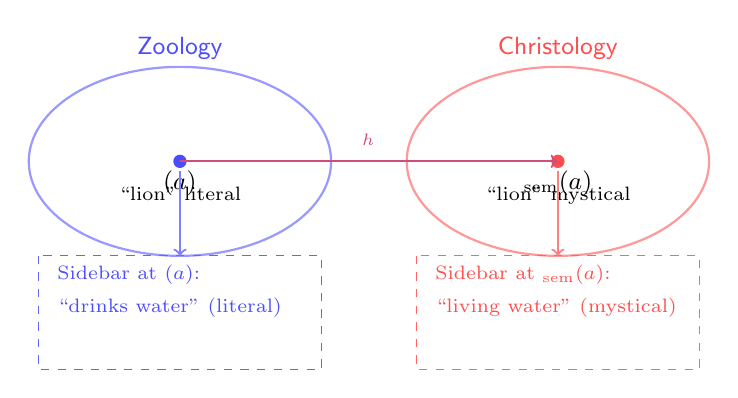
\begin{tikzpicture}[scale=1.2, every node/.style={font=\small}]
  % Zoological basin ellipse
  \draw[thick,blue!40] (-2,0) ellipse (1.6 and 1);
  \node[blue!70] at (-2,1.2) {\textsf{Zoology}};

  % Christological basin ellipse
  \draw[thick,red!40] (2,0) ellipse (1.6 and 1);
  \node[red!70] at (2,1.2) {\textsf{Christology}};

  % Tear (lion in zoology)
  \fill[blue!70] (-2,0) circle (2pt);
  \node[below] at (-2,0) {$\tear(a)$};
  \node[below,yshift=-0.2cm] at (-2,0) {\scriptsize ``lion'' literal};

  % Drift candidate (lion in Christology)
  \fill[red!70] (2,0) circle (2pt);
  \node[below] at (2,0) {$\dtr_{\mathrm{sem}}(a)$};
  \node[below,yshift=-0.2cm] at (2,0) {\scriptsize ``lion'' mystical};

  % Heal edge
  \draw[thick,->,purple!70] (-2,0) -- (2,0) node[midway,above,yshift=2pt] {$\heal_h$};

  % Sidebar pop-outs
  \draw[dashed,blue!60] (-3.5,-1) rectangle (-0.5,-2.2);
  \node[blue!70,anchor=west] at (-3.4,-1.2) {\scriptsize Sidebar at $\tear(a)$:};
  \node[blue!70,anchor=west] at (-3.4,-1.55) {\scriptsize ``drinks water'' (literal)};
  \draw[thick,->,blue!50] (-2,-0.1) -- (-2,-1);

  \draw[dashed,red!60] (0.5,-1) rectangle (3.5,-2.2);
  \node[red!70,anchor=west] at (0.6,-1.2) {\scriptsize Sidebar at $\dtr_{\mathrm{sem}}(a)$:};
  \node[red!70,anchor=west] at (0.6,-1.55) {\scriptsize ``living water'' (mystical)};
  \draw[thick,->,red!50] (2,-0.1) -- (2,-1);

\end{tikzpicture}
\caption{A rupture and heal for ``lion''. At $\tau$ the token is anchored in the
zoological basin. At $\tau'$ a gloss introduces a christological reading, producing
a heal $\heal_h$ in the updated fibre. Sidebars attached to the tear and drift
candidate retarget: the note ``drinks water'' becomes ``living water'' under
transport.}
\label{fig:lion-sidebar}
\end{figure}



\paragraph{Continuing a sidebar conversation.}
If one later wishes sidebars to evolve across time (a tafs\=\i r thread that
persists beyond $\tau'$), the same pattern lifts to DynSem by taking values in a
small univalent universe of presheaves over $y(\tau')$. This yields a displayed
presheaf (a Grothendieck fibration over the time index) but is not needed for
the slice‑local results in this chapter.


\section{Coalgebraic unfolding inside a fibre}
\label{sec:spatial-coalgebra}

Fix \(\tau\). Define the endofunctor
\[
F_\tau\left(X\right) = 
\sum_{x:A\left(\tau\right)} \sum_{s:\mathrm{Simplex}\left(x\right)}\
\sum_{\rho:\mathrm{Witness}\left(s\right)} \Later X,
\]
where \(x\) is a vertex, \(s\) a simplex incident to \(x\), \(\rho\) its witness,
and \(\Later X\) a guarded tail. The final coalgebra
\[
\Traj_{\mathrm{sync}}\left(A\left(\tau\right)\right) = \nu F_\tau
\]
unfolds as \(\unfold\left(x\right)=\left(a,s,\rho,\Later x_1\right)\), disclosing
one in-fibre coherence step at a time. Restriction maps \(r_{\tau,\tau'}\) act
functorially on these trajectories by forgetting simplices not yet present.

\section{Synchronic Witness Log}
\label{sec:swl-sync}

For each \(\tau\) we record in-fibre witnesses in rows
\[
\left(\tau, x, y, \mathrm{tag}, \mathrm{depth}, \mathrm{certificate}\right),
\]
with \(\mathrm{tag}\in\left\{\mathsf{path},\mathsf{homotopy},\mathsf{coherence}\right\}\).
An evidence update that introduces an edge logs a \(\mathsf{path}\) with
\(\Depth=1\); a reconciliation triangle logs \(\mathsf{homotopy}\) with \(\Depth=2\).
Together, SWL and SWL\textsubscript{sync} capture coherence along restriction and
inside fibres with a single depth convention.

\section{Soundness theorem}
\label{sec:soundness-in-slice}

\begin{theorem}[Soundness of repair against embeddings]
\label{thm:full-soundness}
Let \(\left\{E_\tau\right\}\) be embeddings with basins and halo at each \(\tau\).
With restriction maps built by semantic alignment and repairs realised as
evidence-updated fibres, the construction above yields
\(\widetilde A\in \DynSem\) such that:
\begin{enumerate}
\item Temporal rules of Chapter 3 interpret soundly in \(\widetilde A\):
drift as homotopy sections of \(r_{\tau,\tau'}\), rupture as later-slice gluing
with stitches, and reconciliation as higher coherences.
\item In-fibre witnesses interpret as simplices in \(A\left(\tau\right)\) or in
their updated versions \(A^h\left(\tau\right)\): edges for stitches, 2-simplices
for reconciliations, and so on.
\item Rows of SWL and SWL\textsubscript{sync} correspond to genuine homotopy
witnesses: horn fillers added by rupture or overlaps adjoined by evidence.
Depth matches the minimal dimension of the simplex added.
\end{enumerate}
\end{theorem}

\begin{corollary}
\label{cor:repair-sound}
The repair calculus of Chapter 3 is sound for evolving conversational meaning:
an evolving text is a presheaf of Kan spaces whose coherence is governed by one
repair logic, read along restriction and inside fibres.
\end{corollary}
